Next, in order to obtain the desired pathway (Obj.~2) of the transition to the vision, a \emph{backcasting} methodology is used. Backcasting processes are, intuitively, the inverse of forecasts. Instead of extrapolating current trends into the future, they start from a defined end-state or goal that represents a desirable (and somehow plausible) future. Then, either through stakeholder participatory workshops, experts panel consultation or ``in-house''\footnote{Done by the researchers themselves.} processes, a set of intermediate goals are set at whatever time-frames are required. The backcasting process is finalised with the identification of the trends and changes that separate the desired future and the current state of the system under study, as seen in \fref{f:backcasting-methods} \parencite{dreborg1996_Essencebackcasting}. Backcasting usually serves a normative purpose and, most importantly, it is are usually rhetorical in nature, rather than analytical. The strength of this methodology lies in the ability to extend the range of possibilities under consideration \parencite{mcdowall2006_Forecastsscenariosvisions}.

\begin{figure}
\centering
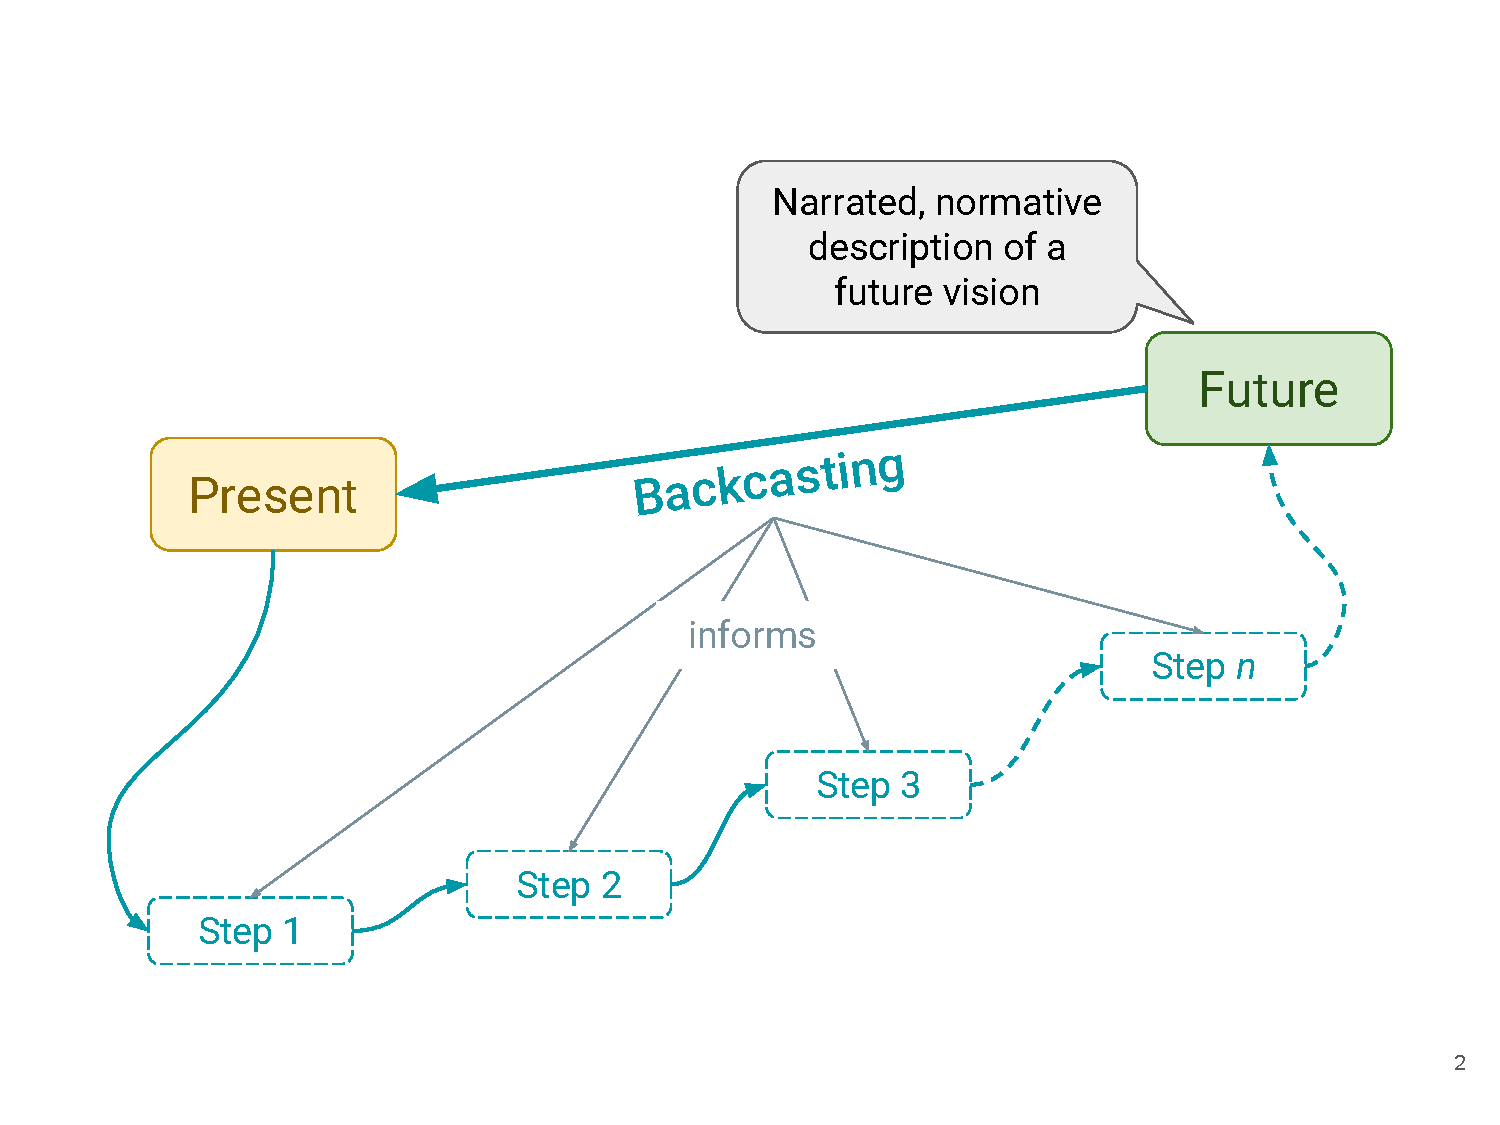
\includegraphics[width=0.7\linewidth,trim=0 2cm 0 2cm,clip]{figures/backcasting.pdf}
\caption[Backcasting framework]{A graphical representation of what the backcasting process entails.}
\label{f:backcasting-methods}
\end{figure}

The main reason behind this method choice is the fact that backcasting is, in itself, a normative methodology for futures analysis \parencite{boerjeson2006_Scenariotypestechniques,mcdowall2006_Forecastsscenariosvisions}, something required for (1) filling the gaps identified by this thesis and (2) to help in the derivation of the policy recommendations for Obj.~4. Additionally, backcasting is also a more promising method when great changes are expected or required \parencite{hoejer2000_Determinismbackcastingfuture}, which is the case of a transition to sustainable mobility. Note that, due to resource limitations and time budgets, the backcasting process is not based in a participatory approach. No stakeholders are involved, nor an expert panel, thus becoming a limitation in the power of the study, as discussed in \cref{c:discussion}. Instead of the participatory approach, the backcasting is based on literature references and insights gained from the IPCC assessment of the SSP1 scenario itself.